\documentclass[11pt]{article}
\usepackage{graphicx,float,subcaption}
\usepackage{xcolor}
\usepackage{amsmath}
\usepackage[margin=1.25in]{geometry}
\usepackage{cleveref}
\usepackage{mathptmx}


\author{Author}
\date{\today}

\begin{document}
\subsection*{A Monte Carlo Study of Clinical Staffing and Patient Scheduling}

We want to compare the expected performance of two scheduling strategies in terms of the patient waiting time and the last patient checkout time. In other words, we want to see if a different patient schedule can result in shorter wait times without lengthening the time the clinic stays open.

To this end, we have constructed a computer model of the clinic patient flow. Assigning reasonable distributions the duration of every patient/clinician interaction, we can simulate many realizations of representative clinic sessions to obtain statistics on the wait and closing times. Here, we fix the number of patients ($n_\text{pt}=12$), clinical teams ($n_\text{ct}=4$), and attending physicians ($n_\text{atp}=2$) at nominal values, and change only the scheduled arrival times (which are subject to a random delay).
\begin{figure}[H]
  
\includegraphics[width=0.75\linewidth]{legend.png}\\[0.5em]
  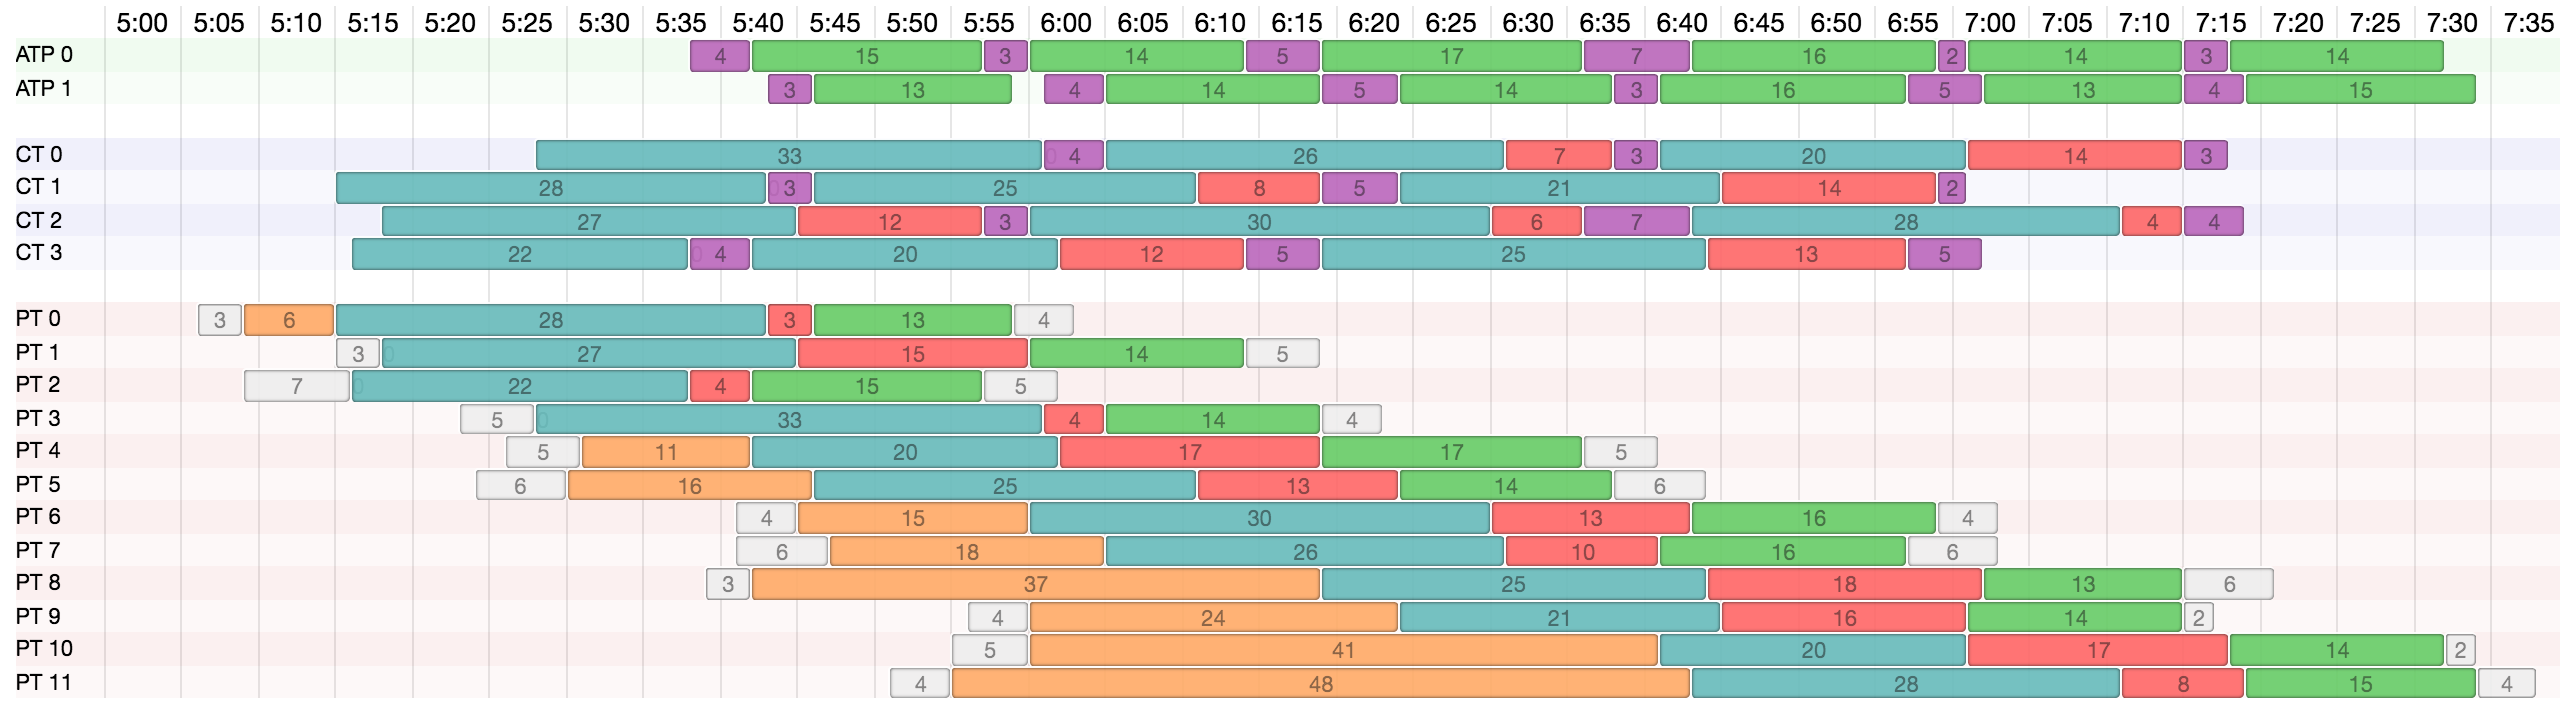
\includegraphics[width=\linewidth]{3_15.png}
  \caption{A typical realization of the simulation model for intervals of 15 minutes between arrivals.}
  \label{fig:gannt-15}
\end{figure}
The current system schedules patients in groups of 3, to arrive at 15 minute intervals. From \cref{fig:gannt-15}, we see that the patients who arrive later experience long wait times due to clinical teams being tied up. This would suggest that increasing the time between arrivals should decrease the amount of patient wating time without increasing downtime or decreasing throughput.
\begin{figure}[H]
  
\includegraphics[width=0.75\linewidth]{legend.png}\\[0.5em]
  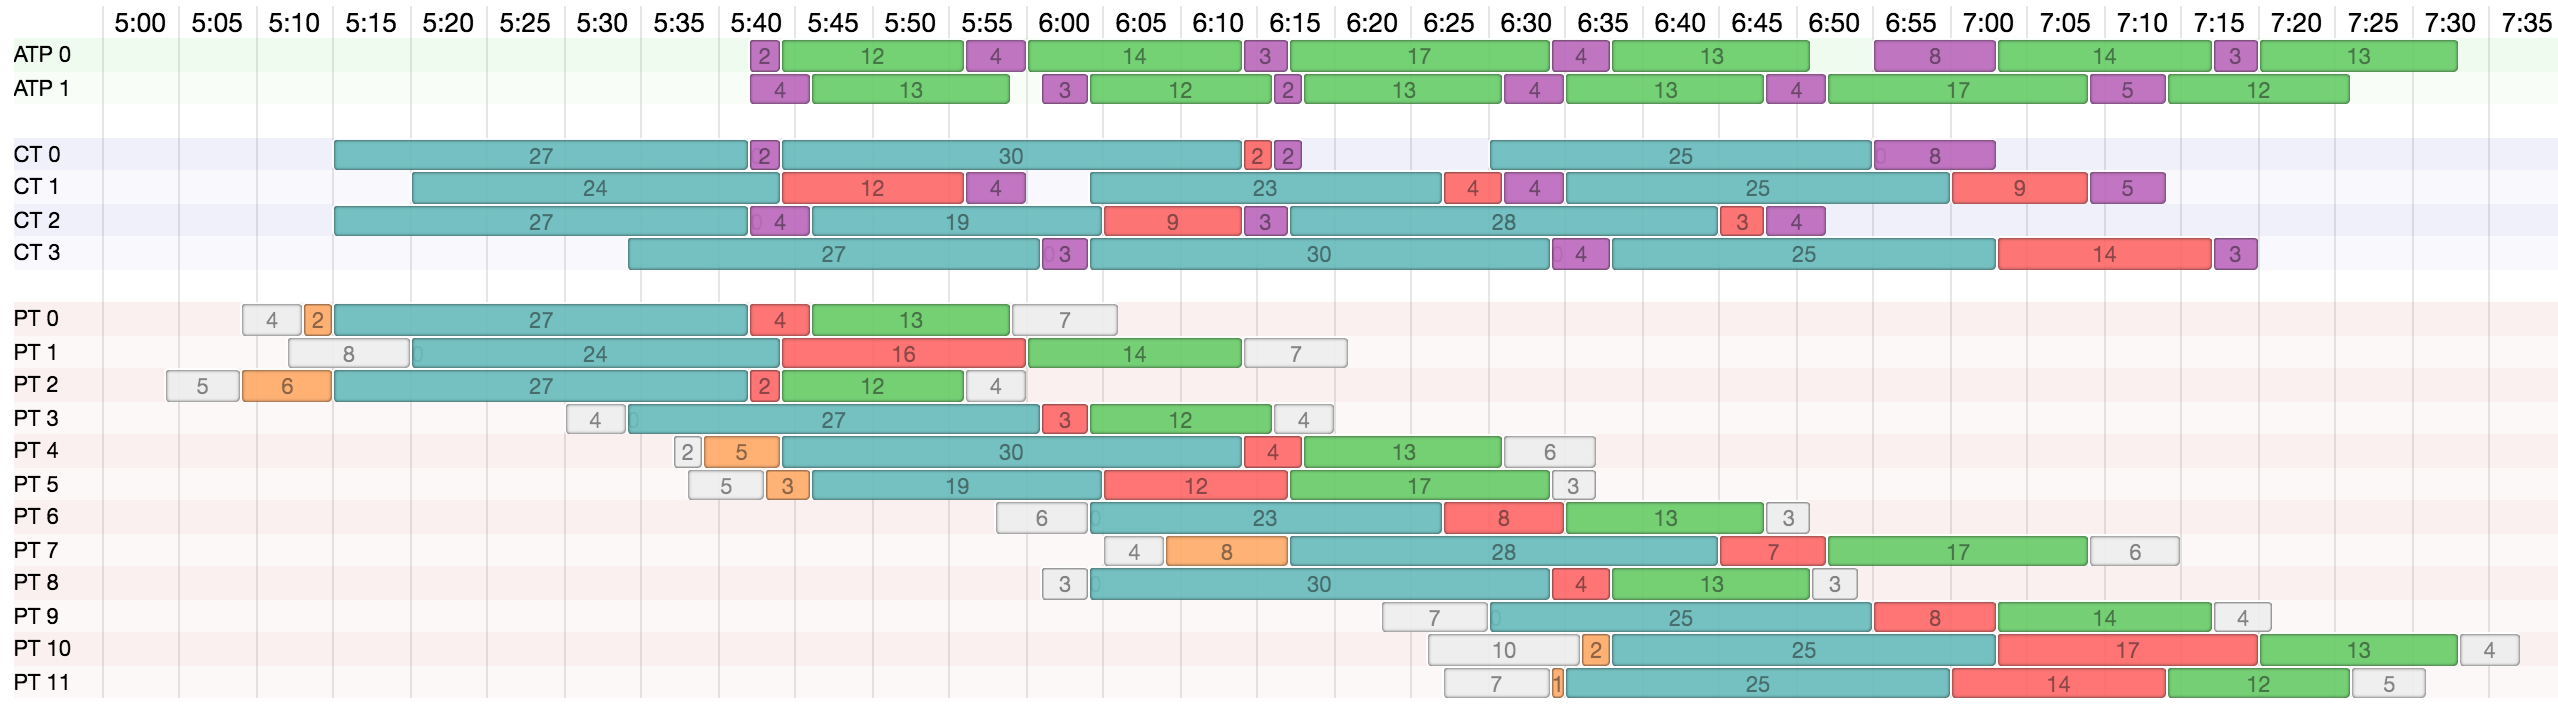
\includegraphics[width=\linewidth]{3_25.png}
  \caption{A typical realization of the simulation model for intervals of 25 minutes between arrivals.}
  \label{fig:gannt-25}
\end{figure}
In \cref{fig:gannt-25}, we see that by increasing the interval to 25 minutes, the amount of orange (patient waiting for clinical team) is significantly reduced, while the schedules of the attendings and clinical teams remain packed with very few gaps, i.e., throughput is not affected and the last patient leaves the clinic at the same time.

We can perform quantitative analysis using Monte Carlo to confirm our observation. We computed 4,000 realizations of clinical sessions using the simulation model, and looked at the distribution of quantities of interest.

In \cref{fig:compare-hist-25}, we see that 75\% of patients will be called within 5 minutes, and 95\% of patients will be called within 15 minutes. Compare this to the existing system, where over 25\% of patients will experience a wait time over 30 minutes, and 5\% of patients will experience wait times of over an hour! We also observe that the clinic closing time is not significantly affected by increasing the interval between patient arrivals to 25 minutes. The average last patient checkout time increases only increases by 2 minutes. However, if we increase the interval to 30 minutes, then from \cref{fig:compare-hist-30}, we see that the last patient checkout time increases by 10 minutes.

\begin{figure}[H]
  \begin{subfigure}[b]{\textwidth}\centering
  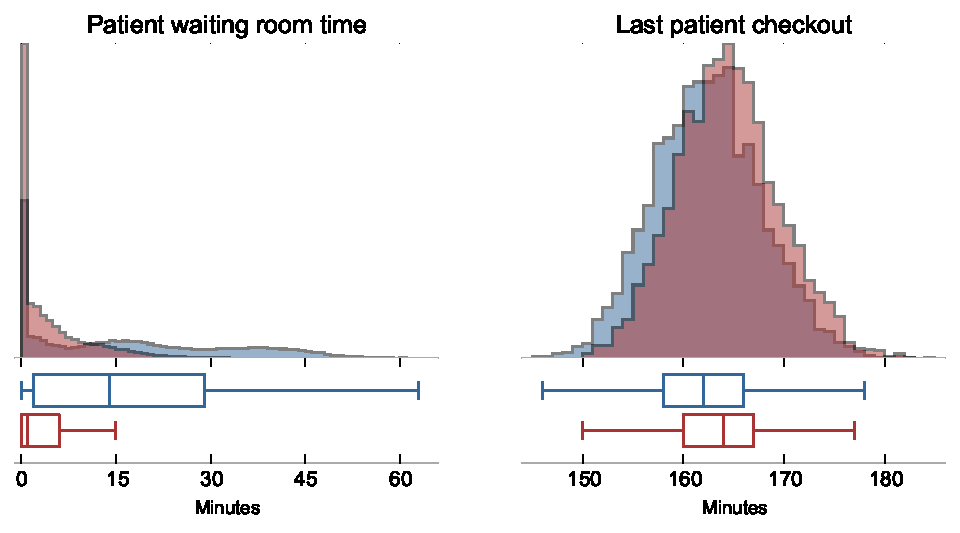
\includegraphics[width=0.8\linewidth]{3_15_3_25_hist1.pdf}
  \caption{\textbf{\textcolor{blue!80!white!60!black}{Blue:}} groups of 3, 15 minutes apart, and \textbf{\textcolor{red!80!white!60!black}{Red:}} groups of 3, 25 minutes apart.}
  \label{fig:compare-hist-25}
  \end{subfigure}
  \begin{subfigure}[b]{\textwidth}\centering
  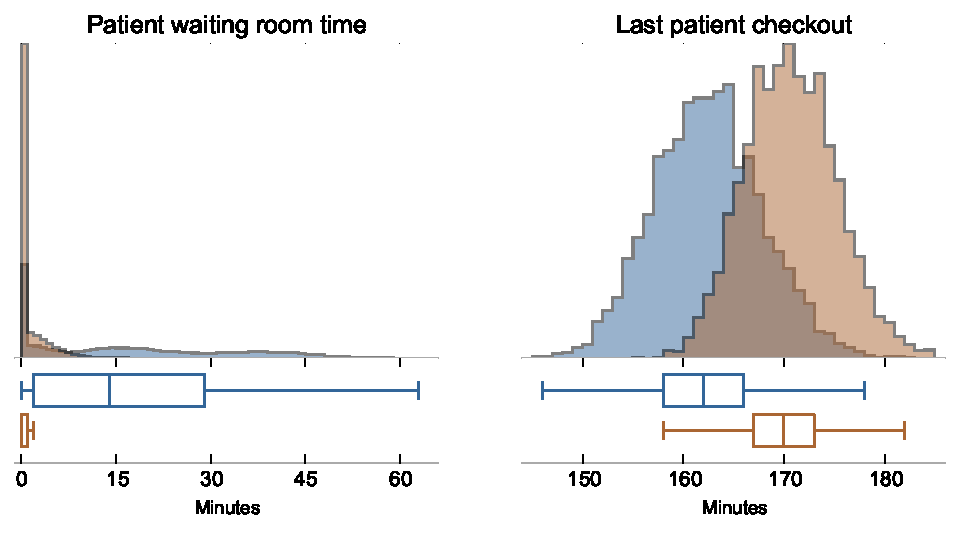
\includegraphics[width=0.8\linewidth]{3_15_3_30_hist1.pdf}
  \caption{\textbf{\textcolor{blue!80!white!60!black}{Blue:}} groups of 3, 15 minutes apart, and \textbf{\textcolor{orange!80!white!60!black}{Orange:}} groups of 3, 30 minutes apart.}
  \label{fig:compare-hist-30}
  \end{subfigure}
  \caption{Simulated distributions of patient waiting room times and last patient checkout times}
\end{figure}
\subsection*{Conclusions and future work}
Based on our simulation model, we would recommend that the interval between patient arrivals be increased from 15 minutes to 25 minutes. However, the accuracy of our model depends on the quality of the parameters that describe the duration of each patient/staff interaction. Here, we used point-estimates based on historical data from a single session, which may not reflect the actual variability across all sessions, and in particular, futures sessions with different clinical teams.

There are many other aspects of scheduling and staffing that may play a role in the operational efficiency of the clinic. By further developing and refining this simulation model, we will be able to ask and confidently answer many questions regarding optimal clinic operation.

\subsection*{Appendix}
Below are some other quantities of interest that were extracted from the simulation.
\begin{figure}[H]
  \begin{subfigure}[b]{\textwidth}\centering
  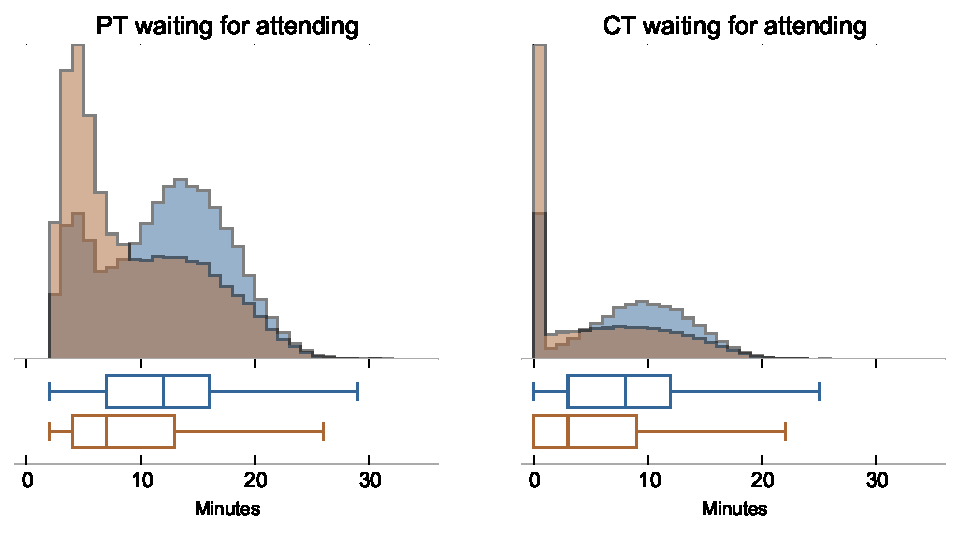
\includegraphics[width=0.85\linewidth]{3_15_3_30_hist2.pdf}
  \caption{\textbf{\textcolor{blue!80!white!60!black}{Blue:}} groups of 3, 15 minutes apart, and \textbf{\textcolor{orange!80!white!60!black}{Orange:}} groups of 3, 30 minutes apart.}
  \label{fig:compare-hist2}
  \end{subfigure}
  \caption{Distributions of patient waiting for attending times and clinical team waiting on attending times. These could be used to inform staffing decisions, as these distributions are most sensitive to the number of clinical teams and attending physicians present. }
\end{figure}
\begin{figure}[H]
  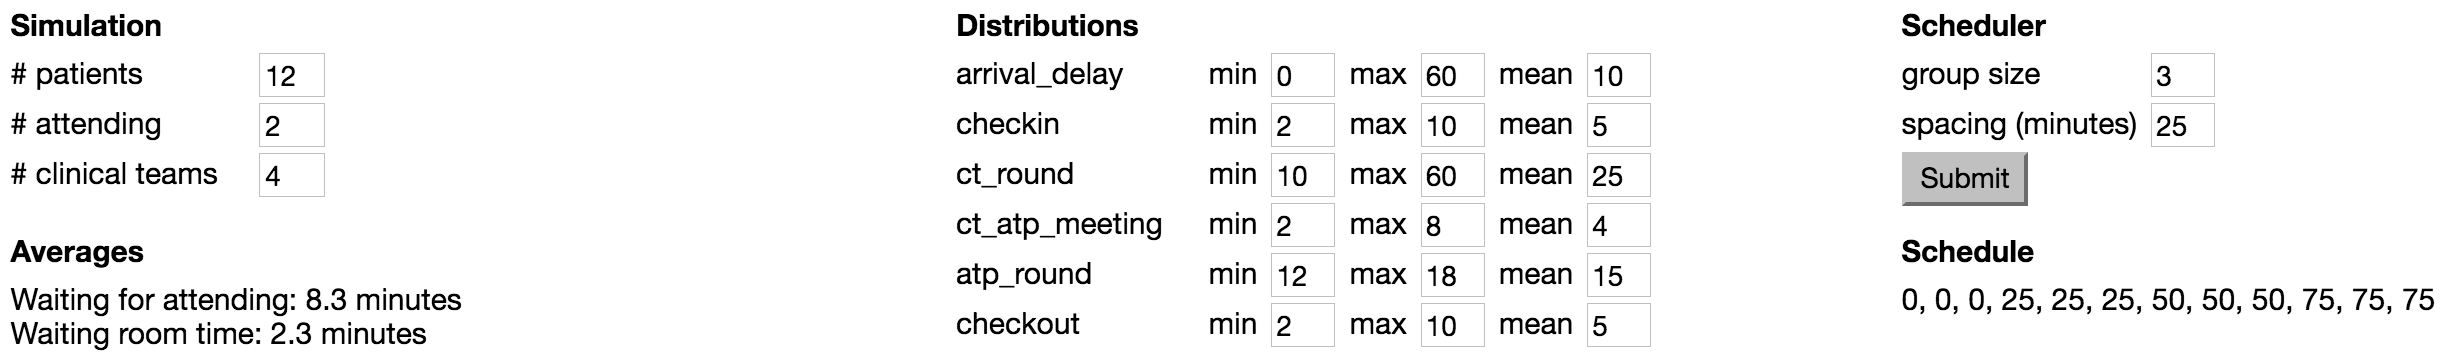
\includegraphics[width=\linewidth]{settings.png}
  \caption{Simulation settings, including distribution parameters for interaction durations}
  \label{fig:settings}
\end{figure}
\end{document}